% #############################################################################
% This is Chapter 5
% !TEX root = ../main.tex
% #############################################################################
% Change the Name of the Chapter i the following line
\fancychapter{Exploring parameters-efficient transfer learning for end-to-end children ASR}
\label{chap:Adapters_exp}
\cleardoublepage

\section{Introduction}
As discussed in the previous chapter, transfer learning emerges as a well-established and effective paradigm for end-to-end ASR.  Despite its effectiveness, we underscored certain limitations that may potentially impede the efficacy of fine-tuning. Notably, challenges arise when fine-tuning large models using a downstream dataset limited in size. This is a crucial issue that requires careful consideration, particularly in light of the recent evolution of ever-growing size of pre-trained model. The use of increasingly bigger models in conjunction with the availability of massive datasets is driving rapid advancements across various domains of machine learning, including NLP and computer vision. In the context of ASR, this scaling up evolution is illustrated by state-of-the-art models such as Whisper and HuBert, where the number of parameters surpass 1 billion.

Some research underscored the interconnected nature of the size of the training dataset and the number of parameters in model, as they both act as mutual bottlenecks in the pursuit of enhancing machine learning models. This critical observation highlight the importance of scaling these two dimensions in tandem for the development of better ASR models. Typically, the augmentation of the model's size results from a combination of an increased number of layers and an expansion of the model's hidden dimensions. As a consequence, the process of fine-tuning specific parts of the model, such as the FFN modules for the Transformer, is intricately linked to the model size, as FFN modules often represents $\frac{2}{3}$ of the total amount of parameters. In addition, TL from the large amount of parameters is storage-inefficient. 

In response to these challenges, the research community has witnessed the emergence of lightweight alternatives, known as parameter-efficient transfer learning (PETL).
%As presented in the previous chapter, transfer learning, despite beeing a well-established and well-performing paradigm has some limitations. Especially when it comes to fine-tuning large models with a limited-size downstream dataset. However, the availability of massive datasets and the development of ever-growing size model allowed rapid progress in many field of machine learning, from NLP, computer vision and ASR. Examples of such models like Whisper and HuBert can go up to more than 1 billion parameters. In addition, the size of the training dataset and the number of model parameters are mutual bottlenecks and must be scaled in tandem, which is a important information for the development of better ASR models.  Usually, the models size are increase by a conjounction of increased number of layer, model's dimension.  As a consequence, fine-tuning part of the model, such as the FFN layers only, can also drasticly increase. 

%More recently, advances on self-supervised learning (SSL)  focused on training models to extract representations from large volumes of unsupervised data. Subsequently, the entire network undergoes fine-tuning to use the extracted representations effectively in supervised tasks. Notably, these advances have led to significant improvements in child speech recognition\cite{9847929,fan2022draft}. However, fine-tuning the entire network in this way can lead to significant computational costs, including long training times and substantial storage requirements. Moreover, SSL is vulnerable to domain shift, when the data domain used for fine-tuning differs from the initial pre-training domain. Although SSL yields improved performances with extensive unlabeled data during pre-training, recent research suggests that even greater improvements can be achieved by including target domain data during the pre-training phase \cite{hwang2022large}.
%However, larger models require more data for effective fine-tuning to prevent over-fitting. 


Residual adapter modules offer an alternative approach to address traditional transfer learning limitations in the context of automatic children's speech recognition of large ASR models. Adapters, specifically designed for Transformer-based systems integrate a compact set of additional layers into a pre-trained source model \cite{houlsby, pfeiffer}. These adapters typically provide enhanced computational efficiency, resulting in faster training and mitigating the problem of catastrophic forgetting. In contrast to conventional transfer learning, where the source model's weights are completely replaced, adapter transfer preserves the backbone model, leaving it unchanged even when the adapter layers are removed. Additionally, due to their limited number of trainable parameters, adapters tend to be less prone to over-fitting.

In this study, we extend research presented in \cite{chen2023efficient} and \cite{10095837} by conducting a comprehensive evaluation of various adapter configurations specifically designed for Conformer models in the domain of children's speech recognition. Furthermore, we introduce a novel adapter configuration, the Two Serial Adapter (TPA). We also perform a comparative analysis between Conformer-based models and traditional Transformer-based models, a comparison that has not been explored in the context of children's speech recognition to the best of our knowledge. Then, considering the potential benefits of age-dependent acoustic models, and given the strong correlation between children's age and acoustic variability \cite{gale2019improving, shivakumar2020transfer}, we propose a novel cluster-based strategy for training adapters. Finally, we explore the data requirements for the Adapter approach compared to traditional fine-tuning.

\section{Adapters}
\begin{figure*}[t]
\begin{center}
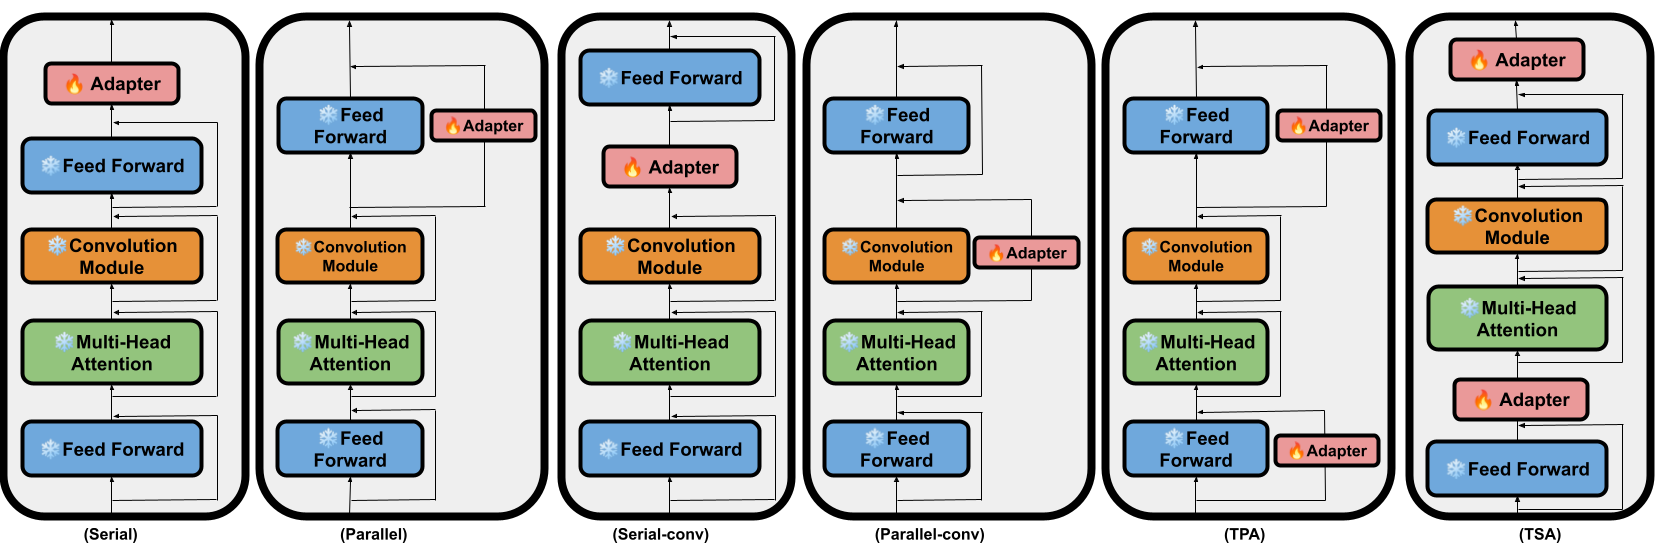
\includegraphics[scale=0.3]{imgs/Adapter_conformer.png}
\caption{Conformer block with various residual adapter configurations.}
\label{fig:all}
\end{center}
\end{figure*}

Adapters were first introduced in the natural language processing field to efficiently adapt large models like Transformers for text classification \cite{houlsby}. They are a simple alternative to full model fine-tuning, adding a small number of parameters at each transformer layer, generally after the feed-forward layer. Adapters use a bottleneck architecture (projection-down followed by projection-up) and have benefits such as parameter efficiency, faster training, and modularity compared to full fine-tuning. Adapter can be expressed as follows:
\begin{equation}
    adapter(x) = x + (W_{up}(f(W_{down}g(x)+b_{down})))+ b_{up})
\end{equation}
where $f(\cdot)$ is the non-linear activation function and  $g(\cdot)$ a layer normalization or identity function.
In terms of computation, Adapters offer faster training as they update fewer parameters. However, they might introduce a slight processing delay compared to fully fine-tuned models at inference, but this difference is typically minimal and can be well-managed \cite{ruckle2020adapterdrop}.

Adapters in the context of children's ASR have received limited attention, with only one notable study by \cite{fan2022draft}, who proposed integrating adapters into self-supervised models and fine-tuning the entire model, including the adapter weights to better model children's speech. In contrast, 
%CAMERA-READY (Remove this)
%, our research distinguishes itself from this prior work.
our primary objective is to update only the adapter weights during supervised training, maintaining the parameter efficiency and modularity of adapters, without relying on semi-supervised pre-training.

\section{Investigating Adapters for children ASR}
In this paper, we investigate the application of Adapters in both Transformer and Conformer architectures. For the Transformer, we examine two integration methods: parallel and serial placement with the Feed-Forward Network (FFN) component \cite{he2021towards}. Within the Conformer architecture, we explore six Adapter configurations, as illustrated in Figure \ref{fig:all}. The first two configurations mirror our Transformer investigation, involving both parallel and serial placements, either after or in parallel with the second FFN layer \cite{chen2023efficient}. Furthermore, we assess the configuration that incorporates an Adapter following the convolution module, referred to as the ``serial-conv'' setup used in \cite{10095837}. Furthermore, \cite{chen2023efficient} introduces two variants of the parallel setup: ``parallel-conv,'' where the Adapter operates in parallel with the convolution module, and ``TPA,'' which deploys two adapters in parallel with both FFN modules in the Conformer layer. 

In the case of serial configurations, we integrate the adapter information with the preceding component denoted as $P$. The specific component $P$ varies depending on the configuration and can be either the FFN or the convolution modules. This integration is accomplished through the following process:
\begin{equation}
    output =  Adapter(P(x))
\end{equation}
In the parallel configurations, the integration process differs slightly. Here, we combine the adapter's output with the output of component $P$ as follows:
\begin{equation}
    output = x + 0.5 * P(x) + (Adapter(x) - x)
\end{equation}
where $x$ is the input of the component $P$. In order to comprehensively explore all feasible configurations, we introduce a novel one called ``TSA,'' which stands for Two Serial Adapters. In this configuration, one Adapter is positioned sequentially after each FFN component.

Additionally, for a comprehensive assessment of Adapter behaviour, we consider four distinct configurations where Adapters are placed in the Decoder. Note that in the Conformer architecture, the decoder is a regular Transformer. Therefore, we initially evaluate the ``Serial''and ``Parallel''setups. Subsequently, we investigate the combination of the most effective encoder Adapter configuration with both Decoder configurations. To the best of our knowledge, there is no prior research that formally investigates the influence of Adapters within an ASR decoder.

% Finally, we explore the use of unsupervised clustering of utterances, motivated by the strong correlation between children's speech variability and age. Our aim is to create clusters of utterances that exhibit similar acoustic characteristics. This process employs a k-means clustering algorithm on the x-vector representation \cite{snyder2018x} of each training utterance. The primary objective is to investigate whether Adapters trained on comparable speech characteristics yield improvements over a general Adapter on the entire training set. To evaluate this approach, we use this clustering in the test set, where test utterances are decoded with their respective cluster Adapters.
Finally, motivated by the strong correlation between children's speech variability and age, we investigate the possibility of 
training specialized Adapters for groups of speakers exhibiting similar acoustic characteristics based on unsupervised clustering. In practice, we apply a k-means clustering algorithm on the x-vector representation \cite{snyder2018x} of each training utterance. Then, a different adapter model is trained for each  speaker cluster. During test, the closest speaker cluster is found for each test utterance and the corresponding Adapter weights are used for decoding.
The primary objective of these experiments is to investigate whether Adapters trained on comparable speech characteristics yield improvements over a general Adapter on the entire training set. 

\subsection{Relation to prior work}
\label{sec:prior}
% No work fully compared Adapter vs Conformer in Children speech
Children's speech is inherently atypical and displays a significant degree of variability, making it imperative to assess the efficacy of existing methods in modelling children's speech. This paper introduces several contributions to the field of automatic children's speech recognition. Firstly, the paper conducts a comparative analysis between traditional Transformer and Conformer-based models. Secondly, we propose the use of residual adapters to tackle the challenges associated with children's ASR in large models. This study conducts a comprehensive and systematic evaluation of various adapter configurations designed explicitly for Conformer models extending prior work \cite{chen2023efficient,10095837}, pinpointing the most effective setups for children's ASR tasks. Indeed, in prior work different configurations were employed resulting in a lack of standardised evaluation. Additionally, a new adapter configuration called the Two Serial Adapter (TSA) is proposed to cover all conceivable configurations. Furthermore, to the best of our knowledge, there has been no work exploring Adapters in the decoder of an ASR model. Lastly, a cluster-based training strategy is proposed as an innovative approach to further enhance children's ASR by leveraging speaker-dependent acoustic characteristics. Altogether, these contributions advance the state of children's ASR and provide valuable insights for future research in this domain. 

\section{Implementation details}

All experiments were performed using the SpeechBrain toolkit \cite{speechbrain}. We used  12 Transformer or Conformer layers for the encoder, for the Transformer and Conformer model respectively, and 6 Transformer layers for the decoder, all with dimensions 512. These models have been pre-trained using the LibriSpeech dataset \cite{librispeech} and are publicly available\footnote{https://huggingface.co/speechbrain/asr-transformer-transformerlm-librispeech} \footnote{https://huggingface.co/speechbrain/asr-conformer-transformerlm-librispeech}. Furthermore, for all of our experiments, we used the same Transformer language model, trained on 10 million words 
%CAMERA-READY (Add Information about the Language model training)
on the LibriSpeech transcriptions.
The adapter architecture consists of a  first linear layer projection to dimension 512 with a ReLu activation, followed by another linear layer projection to dimension 512 with a residual connection of the adapter input. 
%CAMERA-READY (Comemnt this)
%We would like to emphasise that previous research has investigated the exploration of hidden-dimension size, consistently demonstrating that larger dimensions tend to yield improved performance scores \cite{chen2023efficient}. 
%CAMERA-READY (Instead this:)
The use of a hidden-dimension size equal to the model size (instead of a bottleneck) was motivated by previous research exploring hidden-dimension size, that consistently demonstrated that larger dimensions tend to yield improved performance scores \cite{chen2023efficient}.
All models were trained for 30 epochs, with a learning rate of $8\cdot10^{-4}$ for Adapters experiments and of $8\cdot10^{-5}$ for fine-tuning the entire model.
%CAMERA-READY (Add information about the training)
For the clustering experiments, we use the k-means clustering algorithm on the speaker-embedding of each utterance. The speaker embeddings were extracted using a publicly pre-trained ECAPA-TDNN model, trained on adult speech\footnote{https://huggingface.co/speechbrain/spkrec-ecapa-voxceleb}.

\section{Results}
\label{sec:results}

\subsection{Configurations}
\begin{table}[t]
\caption{Results of the different Adapters configurations in both Transformer and Conformer.}
\begin{center}    
\begin{tabular}{ccc}
\hline
 Method & WER     & Trained params    \\ \hline \hline
\multicolumn{3}{c}{Transformer} \\ \hline
\multicolumn{1}{l}{\textit{Frozen}} & 25.04\%   & - \\
\multicolumn{1}{l}{\textit{Full fine-tuning}} & 12.99\% & 71.5M \\ \hline
\multicolumn{1}{l}{Serial}  &   12.78\% & 6.3M  \\ 
\multicolumn{1}{l}{Parallel}  &     \textbf{12.62\%} & 6.3M  \\ \hline\hline
\multicolumn{3}{c}{Conformer} \\ \hline
\multicolumn{1}{l}{\textit{Frozen}} & 21.75\%   & - \\ 
\multicolumn{1}{l}{\textit{Full fine-tuning}} & 12.28\% & 109.1M \\ \hline
\multicolumn{1}{l}{Serial}  &   11.76\% & 6.3M  \\ %11.84 
\multicolumn{1}{l}{Serial-Conv} & 11.78\%     & 6.3M  \\
\multicolumn{1}{l}{Parallel}    & 11.72\% & 6.3M  \\ % 11.88 
\multicolumn{1}{l}{Parallel-conv} & 11.79\%      & 6.3M  \\ %\hline
\multicolumn{1}{l}{TPA} & \textbf{11.58\%}     & 12.6M  \\ %11.85
\multicolumn{1}{l}{TSA} & 11.75\%     & 12.6M  \\ \hline %11.72
\multicolumn{1}{l}{Serial (Decoder)} & 18.09\%     & 3.2M  \\ 
\multicolumn{1}{l}{Parallel (Decoder)} &17.76\%     & 3.2M  \\ \hline
%\multicolumn{1}{l}{TPA + Serial (Decoder)} & 00.00(T)\%     & 15.8M  \\
%\multicolumn{1}{l}{TPA + Serial (Decoder)} & 11.68\%     & 15.8M  \\ 
\multicolumn{1}{l}{TPA + Parallel (Decoder)} & \textbf{11.47\%}     & 15.8M  \\ \hline

\end{tabular}
\end{center}

\label{tab:res}
\end{table}

In this section, we present a comprehensive evaluation of Adapter configurations applied to both Transformer and Conformer models, assessing their performance based on Word Error Rate (WER), as presented in Table \ref{tab:res}.  First, we assess 
%CAMERA-READY ( remove this to make more clear that frozen is no-finetune and without adapters)
%Adapter configurations in 
the Transformer model when no fine-tuning was applied (\textit{Frozen}), resulting in a WER of 25.04\%. Conversely, \textit{Full Fine-Tuning} involved complete fine-tuning of the entire model,
%CAMERA-READY (Make more clear that this is our baseline)
working as our baseline system
, reducing the WER significantly to 12.99\%, at the expense of 71.5 million trainable parameters.
Turning to the Adapter setups, we investigate the ``Serial'' and ``Parallel'' configurations, both equipped with 6.3 million trainable parameters. The ``Parallel''emerged as the best configuration, achieving the lowest WER of 12.62\% compared to 12.78\% for the ``Serial``. These results underscore the effectiveness of Adapter configurations within the Transformer architecture, as they both perform slightly better than the full-finetuning.

Next, we investigated the Conformer model, we once again explored \textit{Frozen} and \textit{Full Fine-Tuning}. In \textit{Frozen} the pre-trained model remained untouched, yielding a WER of 21.75\%. The Full fine-tuning, in a similar way as the Transformer, led to enhanced performance, reducing the WER to 12.28\% with a total of 109.1 million trainable parameters. We can observe that given the same pre-training dataset, the Conformer architecture outperforms the regular Transformers. Within the set of adapter configurations, ``Serial'' achieved a WER of 11.76\%, while ``Parallel'' demonstrated slightly better performance with a WER of 11.72\%. These results indicated that ``Parallel''Adapters were more effective in improving WER in the Conformer model. When Adapters are placed after the convolution layer, with the ``Serial-conv'' and ``Parallel-conv'' configuration, both slightly under-perform compared to Adapters placed after the second FFN component with respective scores of 11.78\% and 11.79\%. Finally, we evaluated the ``TPA''and ``TSA''configurations. The ``TPA''configuration emerged as the most promising, with a very remarkable WER of 11.58\% using 12.6 million trainable parameters, while ``TSA''achieved a WER of 11.75\%, which is slightly under-performing compared to the ``TPA''configuration.

In addition, we evaluated the use of  Adapters in the decoder. As the decoder of the Conformer architecture is a regular Transformer, we only evaluate the ``Serial''and ``Parallel'' setup, which respectively reached 18.09\%  and 17.76\% WER with 3.2 million parameters. Results showed that Adapters are more relevant when plugged into the encoder. It confirms that acoustic variability plays a critical role in the degradation of children's ASR performance. Finally, combining ``TPA''in the encoder layers with ``Parallel''Adapters in the decoder outperforms Adapters in the encoder only, with 11.47\% WER. Consequently, this configuration stands as the most effective model. 

%CAMERA-READY (Add small paragraph on the statistical test)
We performed statistical tests (Matched Pairs Sentence-Segment Word Error) across all Adapter setups in comparison to the full fine-tuning configuration using SCTK, the NIST Scoring Toolkit \footnote{https://github.com/usnistgov/SCTK/tree/master}. 
%ALBERTO - Add a referene or link to this toolkit
The results reveal that, in all scenarios, the \textit{p}-value is less than or equal to 0.001. This observation denotes statistical significance, indicating evidence against the null hypothesis. 

These results collectively illustrate the versatility and effectiveness of different Adapter configurations within the Transformer and  Conformer model for the children's ASR task. ``TPA''Adapters in the Encoder combined with ``Parallel''Adapters in the Decoder showcased outstanding performance, highlighting their potential as a fine-tuning replacement in large model children ASR scenarios.

\subsection{Unsupervised Clustering of utterances}
\begin{table}[t]
\caption{Results of the clustering approach.}
\begin{center}    
\begin{tabular}{cc}
\hline
  \# of clusters & Average WER     \\ \hline
\multicolumn{1}{c}{1} & 11.58\%  \\% OR 11.70%  If we consider 40 epochs instead of 30 here
\multicolumn{1}{c}{2} & \textbf{11.50\%}  \\
\multicolumn{1}{c}{3} & 11.57\%  \\
\multicolumn{1}{c}{4} & 11.51\%  \\ \hline 

\end{tabular}
\end{center}

\label{tab:res_clusters}
\end{table}



In this section, we present the outcomes of our clustering approach, as summarised in Table \ref{tab:res_clusters}. We investigated the influence of varying cluster numbers on ASR performance, ranging from 1 to 4 clusters using the ``TPA''in the encoder-only configuration. Notably, when the data remained unclustered (one cluster), the ASR system exhibited a WER of 11.58\%. However, the two-cluster configuration surpassed the others, achieving a superior performance of 11.50\%. This result suggests that partitioning the data into two distinct clusters enables the Adapters to more effectively capture underlying patterns intricately linked to their respective clusters, consequently enhancing the recognition scores. Furthermore, we explored the impact of increasing the number of clusters to three and four, revealing only marginal differences in performance, with WERs of 11.57\% and 11.51\%, respectively. These findings underscore the role of data clustering in children's ASR systems.

\section{Additional parameter-efficient procedures}
\begin{figure}
    \begin{center}
        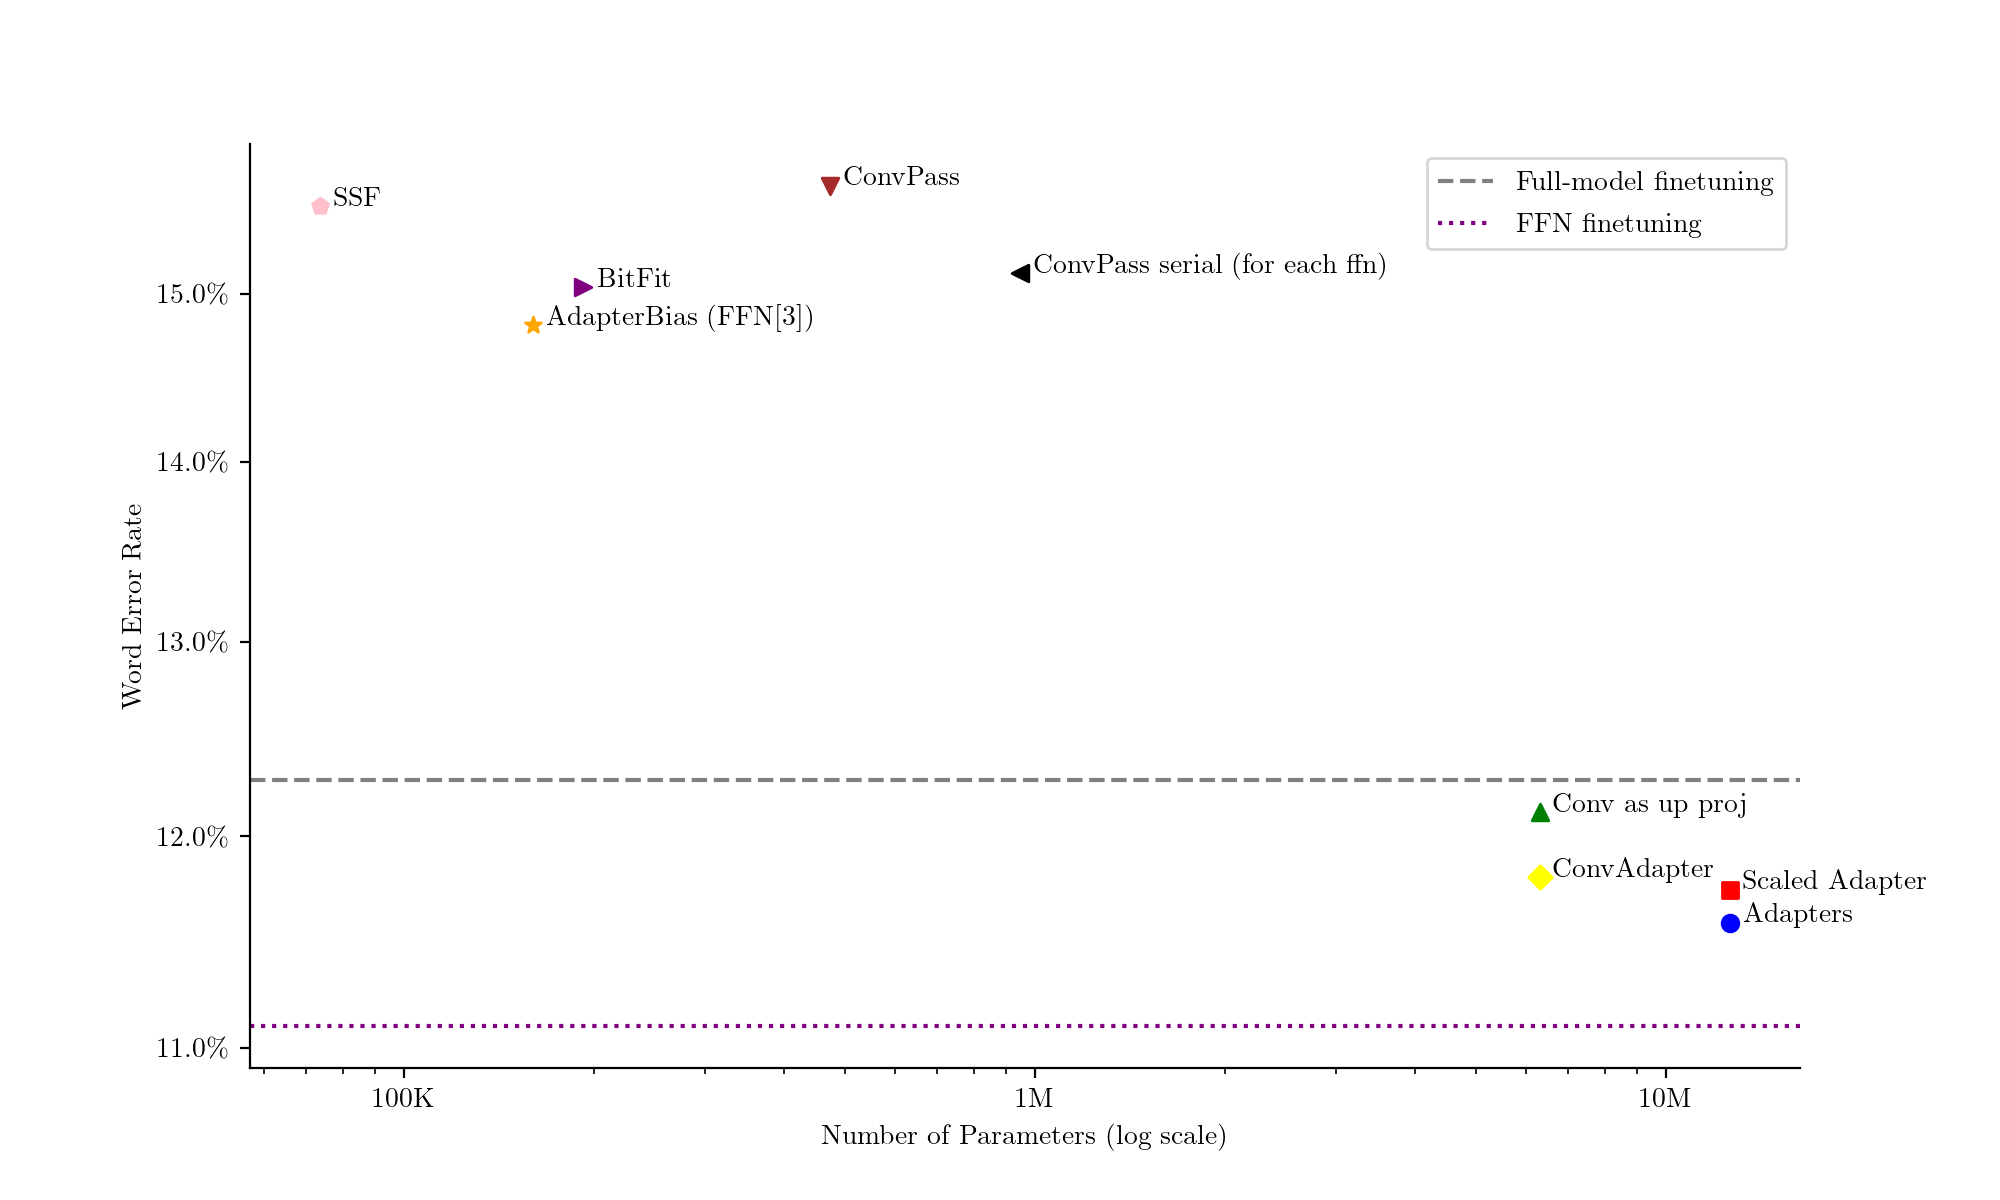
\includegraphics[width=\textwidth]{imgs/Adapter_compare_withoutWide.png}
        \caption{Different paramter efficent procedure for children ASR in conformer model}
        \label{fig:adapter_compared_withoutWide}
    \end{center}
\end{figure}
\subsection{Scaled Adapters}
\subsection{Convolution based Adapters}
\subsection{BitFit}
\subsection{Scale and Shift features}
\begin{align}
    y = \gamma \odot x + \beta
\end{align}
\subsection{AdapterBias}
\section{Shared Adapter}
\begin{figure}
    \begin{center}
        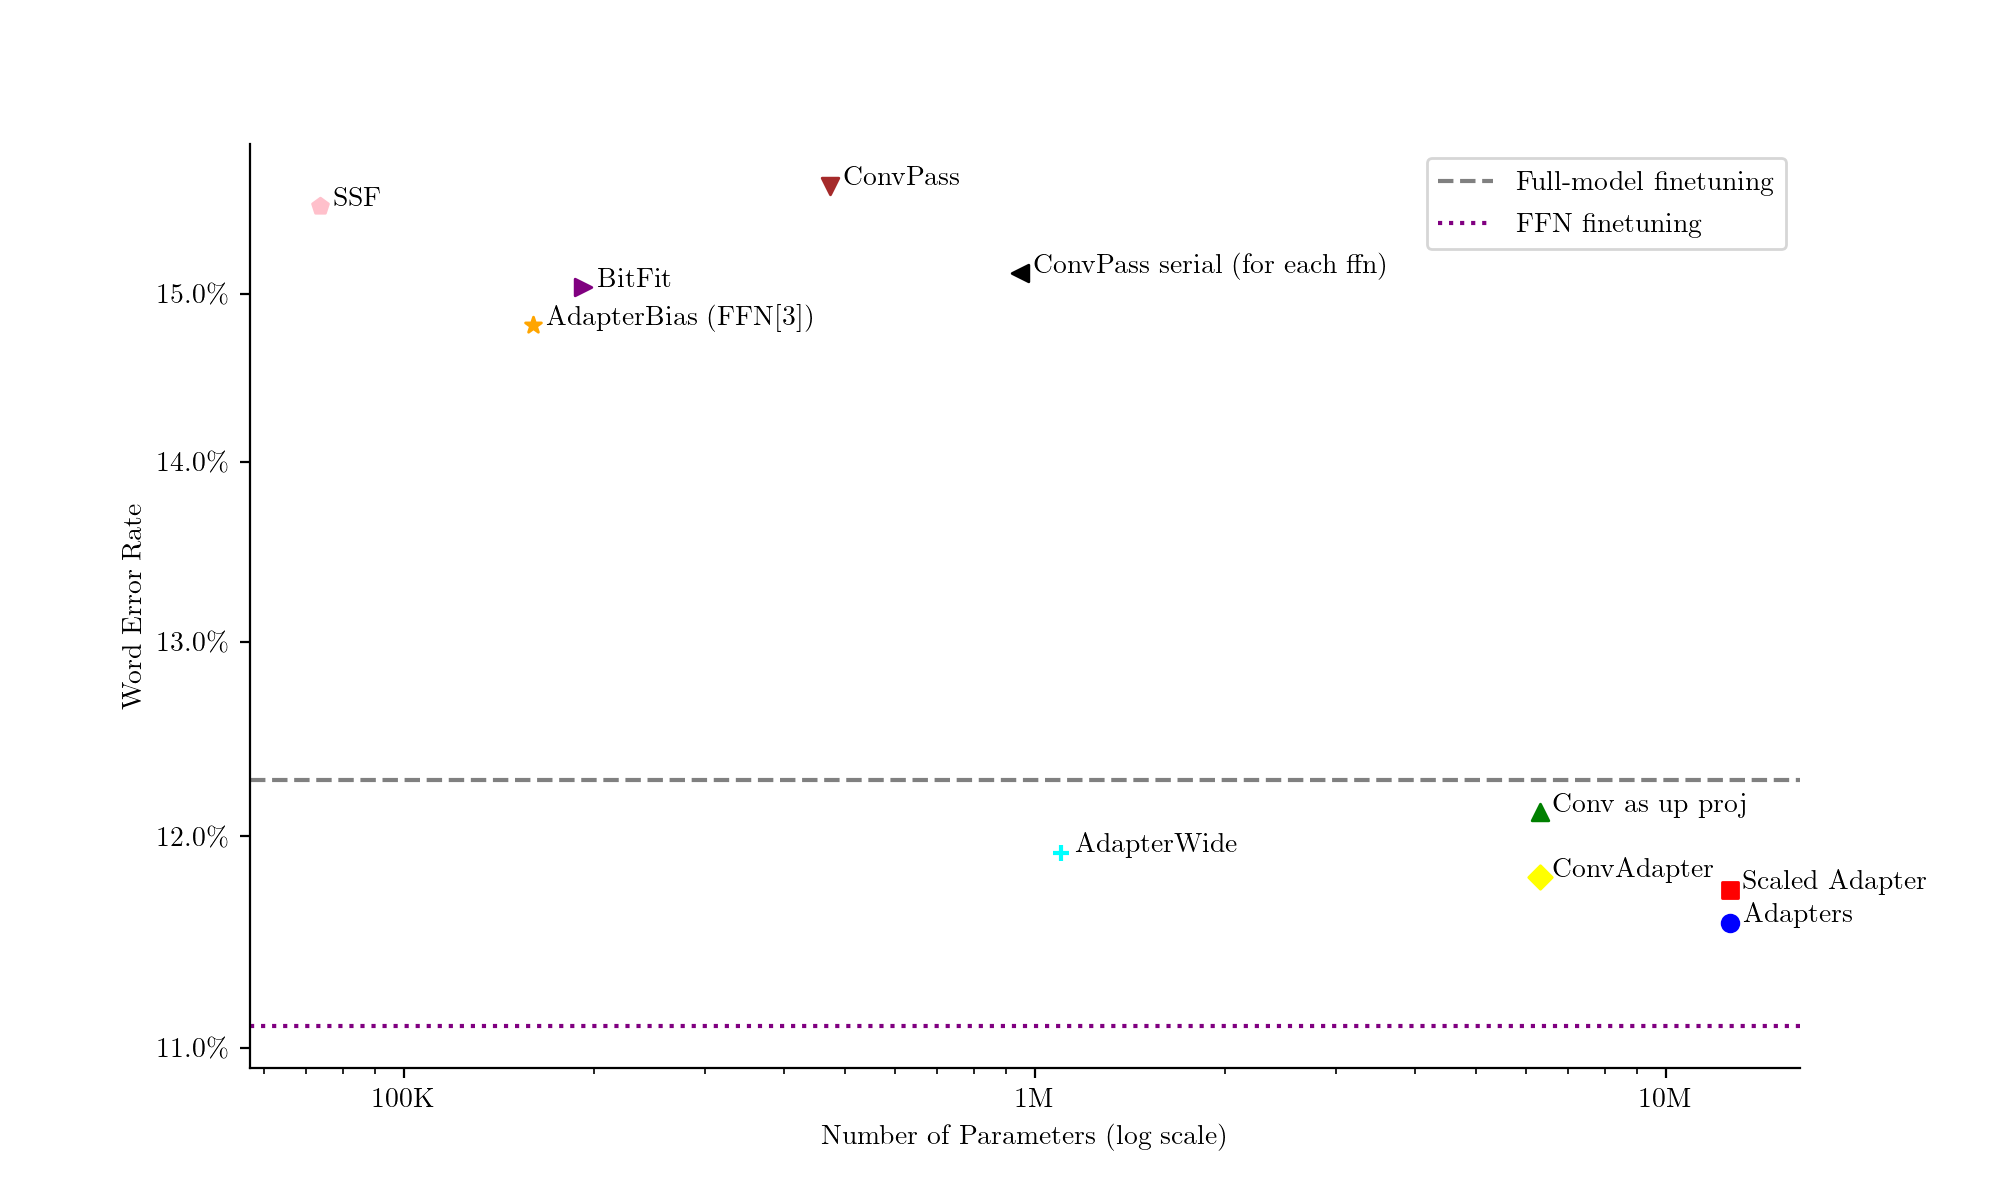
\includegraphics[width=\textwidth]{imgs/Adapters_compare.png}
        \caption{Different paramter efficent procedure for children ASR in conformer model with shared-Adapters}
        \label{fig:adapter_compared}
    \end{center}
\end{figure}



%  SSL

The final research direction we want to explore in this thesis is self-supervised learning (SSL) as a front-end feature rather than typical filter banks or MFCCs. For these models, the training process is separated into two stages. The first phase of training is self-supervised, which implies that no labels are used during training. The objective of this first phase is to present a large amount of unlabelled data to the system so that it learns a good speech representation. The second stage of learning is supervised fine-tuning, in which the model is taught to predict specific phonemes using the robust representation acquired in the previous stage with the help of a small amount of labelled data. In this category, two models stand out as state-of-the-art: Wav2Vec 2.0 \cite{baevski2020wav2vec} and HuBert \cite{hsu2021hubert}. As a preliminary experiment, to asses the usability of such frameworks for children ASR, we trained a BiLSTM model using the output of a variety of frozen self-supervised systems. For this experiment we used a subset of 50h of the Myst corpus \cite{MyST}, and the preliminary findings are displayed in the table \ref{tab:ssl}
\begin{table}[ht]
\centering
\begin{tabular}{lcc} 
\hline
Front-end & UER & WER \\ 
\hline
Fbanks & 12.29\% & 35.14\% \\ 
\hline
TERA \cite{tera} & 11.31\% & 31.80\% \\
Audio Albert \cite{chi2021audio} & 12.28\% & 34.69\% \\
Wav2Vec2.0 Base & 7.37\% & 19.76\% \\
Wav2Vec2.0 Large~ & 7.00\% & 18.76\% \\
Distill HuBert \cite{chang2022distilhubert} & 9.22\% & 25.75\% \\
HuBert Base & 7.40\% & 19.77\% \\
HuBert Large & \textbf{6.03\%} & \textbf{15.41\%} \\
\hline
\end{tabular}
\caption{Results without language model of Self-supervised front-end}
\label{tab:ssl}
\end{table}

Where Base, and Large represent the same model with different number of parameters (in the order Base $<$ Large).
Even though we did not use a language model in this pilot experiment, the results are of the same order as those reported in section \ref{section:exp} obtained with a transformer and a transformer language model. Such results demonstrate that SSL learns substantial speech characteristics. For future research, we aim to explore in depth what information is encoded in SSL models and why they work well on children, and how we may use this knowledge to enhance children's ASR.
